\Chapter{Táblás játékok specifikációja}

%(6-8 oldal)

% TODO: Felsorolni a játékokat, és külön alpontokban leírni a szabályrendszerüket formálisan.
% Itt kellene megadni, hogy mi és milyen formában lehet bennük személyre szabható.
% Szabályok, szabály változatok
% Matematikai jellegű leírások kellenének ide
% Ellenőrzések leírása elvi szinten (például indexelési módok, tábla reprezentáció)

\Section{Általános leírás}

A projekt célja egy olyan webalkalmazás elkészítése, ahol emberek emberek ellen játszhatnak klasszikus két személyes társasjátékokat. A játék a játékok webes felületen, böngészőben, telepítés nélkül használhatóak lesznek.

Az alkalmazásban megtalálható játékok:
\begin{itemize}
	\item amőba,
	\item dáma
\end{itemize}

A játék különlegességét az adja, hogy előre definiált opciókat kiválasztva a játékosok megváltoztathatják a játékszabályokat. A játék így humoros, izgalmas helyzeteket teremthet.

Az oldalon csak regisztrált felhasználók játszhatnak. A regisztráció előnye, hogy a felhasználó az általa megadott névvel szerepelhet a játékban, ill. statisztikákat, rangsorokat lehet összeállítani. A felhasználó saját statisztikái segíthetik a többi játékost a megfelelő partner kiválasztásában. Pl. képet kaphatnak az ellenfél erősségéről. A rangsorok egyrészt érdekesek, másrészt meghozzák a kedvet a versengéshez, a még több játékhoz.

Az alkalmazás egyik menüpontjában pedig találunk majd bemutatkozó leírást, az eredeti játékok szabályzatát, leírást a lehetséges változtatásokról, és lehetőséget a kapcsolatfelvételre (email formájában) észrevételek, hibák bejelentésére. 

\Section{Amőba}

\SubSection{Játékszabály}
Az amőba a legismertebb és legegyszerűbb táblás játékok egyike. Általában négyzetrácsos papíron játsszák. A négyzetháló mérete lehet egyenlő a rendelkezésre álló papír méretével, de kisebb terület is kijelölhető.

Menete: A játékosok felváltva helyeznek egy-egy jelet a tábla valamelyik, még üres négyzetébe. Mindenki a saját jelével játszik. (A leggyakoribb jelek az X és az O.) Az nyer, akinek sikerül saját jeleiből ötöt egyenes vonalban - vízszintesen, függőlegesen vagy átlósan - egymás mellé helyeznie. \cite{fiveinarow-rules}
%forrás: http://mek.niif.hu/00000/00056/html/132.htm

\SubSection{Személyre szabhatóság}
Személyre szabhatóság szempontjából a legjobb alapanyag. Nézzük is, mi mindennel lehet feldobni!
\begin{itemize}
	
	\item Tiltott mezők:
	
	A pályán olyan mezőket helyezünk el véletlen szerűen, amelyre nem rakhatunk karaktert.
	\item Csapda mezők:
	
	A pályán olyan mezőket helyezünk el véletlen szerűen, amelyekre, ha karaktert tesznek, a mező bepirosodik pár másodpercre és a karakter nem kerül kirajzolásra (végez vele a csapda). Ez után a kör átadódik a másik játékosnak. A csapda aktiválódása után a mező semlegessé válik, tehát ugyan úgy lehet rá karaktert tenni, mint bármelyik üres mezőre.
	\item Eltüntető karakter
	
	A játék kezdetekor mindkét játékos kap néhány különleges karaktert, amelyet letéve "kiradírozhat" 1 vagy 5 több karaktert a pályáról.
	\item Eltűnő karakterek:
	
	Minden 3-5 kör után mindkét játékosnak eltűnik egy-egy véletlen szerűen kiválasztott karaktere.	
	\item Elhelyezhető csapdák
	
	A játék kezdetekor mindkét játékos kap néhány karaktert, amelyet letéve csapdát helyezhet el.	
\end{itemize}

\SubSection{Tábla reprezentáció}\label{board-repr}

A táblának a megrajzolása egyszerű, csak egy négyzetrácsra van szükség (továbbiakban vászon). A mezők számontartása és indexelése már érdekesebb. Esetünkben egy három dimenziós objektumban rögzítjük a mezőket. Első dimenzió reprezentálja az x sorindexet a vízszintes léptetéshez, második dimenzió az y oszlopindexet függőleges léptetéshez, a harmadik pedig a szükséges adatokat tartalmazó objektumokat jelenti. Szemléletesebb megfogalmazásban lesz egy tömbünk, ami tömböket tárol, amikben adat objektumok lesznek. Ezekben az adat objektumokban tároljuk el a mező koordinátáit a vásznon, a mező állapotát számmal jelölve, és szükség esetén bármilyen a mezőre vonatkozó információt. Egy tábla elvi megjelenítését mutatja be a \ref{fig:field-repr} ábra.

\begin{figure}[!h]
	\centering
	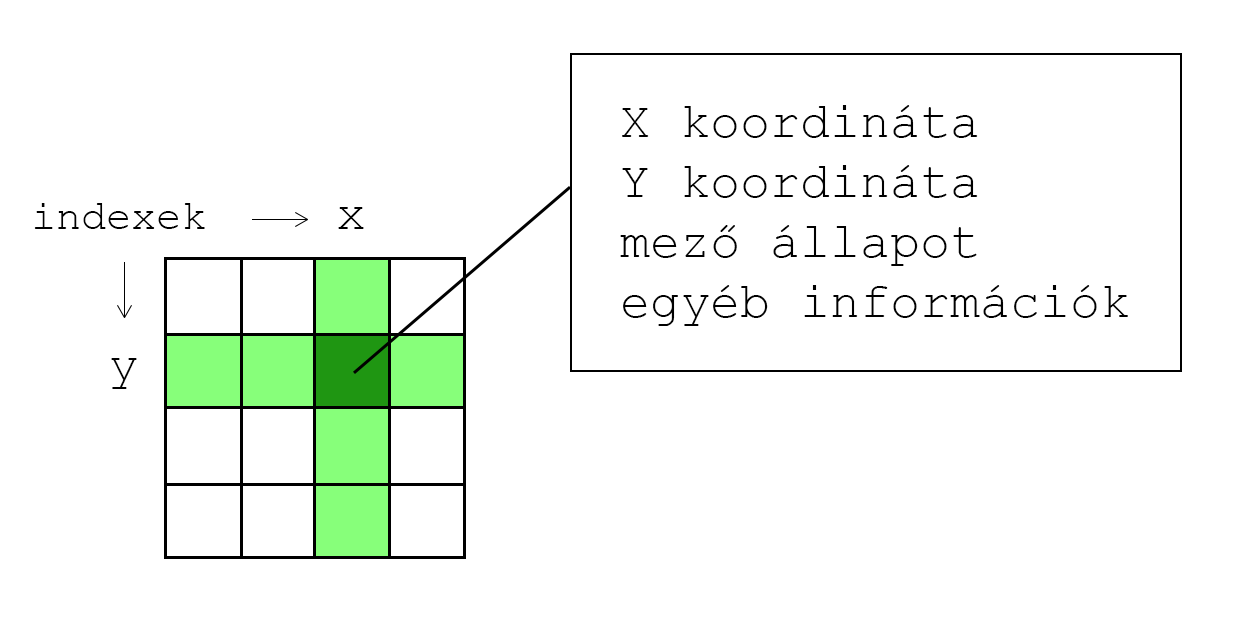
\includegraphics[width=0.6\linewidth]{kepek/field-representation.png}
	\caption{\textit{Tábla reprezentáció}}
	\label{fig:field-repr}
\end{figure}

A mezők állapotai az alábbiak lehetnek:
\begin{itemize}	
	\item 0 - semleges
	\item 1 - kezdő játékos
	\item 2 - másik játékos
	\item 3 - tiltott mező
	\item 4 - csapda mező
\end{itemize}

Fontos különbséget tennünk az index és a koordináták között. Az index az elméleti, a koordináták a fizikai elhelyezést jelölik. Utóbbi a kirajzoláshoz szükséges.

Tehát a 2. sor 3. oszlopában található mező állapotára így hivatkozhatunk: mező[3][2].állapot.

\SubSection{Szabály ellenőrzés}

Az első dolog, amit meg kell vizsgálnunk, amikor egy játékos letesz egy karaktert, a mező állapota. Ilyenkor lekérjük a kiválasztott mező indexeit, majd ez alapján kikeressük a mező értékeinket tároló objektumból a mező állapotát. Ha a mező semleges, kirakjuk a mezőre a karaktert. Ha csapda, akkor annak megfelelően járunk el. Ha már egy játékos karakterét tartalmazza, vagy a mező tiltott, nem történik semmi, nem kerül ki a karakter, a játékosnak másik mezőt kell választani.

Ha sikerült kitenni a karaktert, ellenőriznünk kell, hogy nem nyert -e a játékos. Ránézésre ugyan nyilván való, és egy szempillantás alatt látszik az eredmény, de hogy magyarázzuk el a számítógépnek?

A nyertes kombinációk kijöhetnek vízszintesen, függőlegesen, vagy átlósan (ebből kettő is van). Tehát ezeket a vonalakat kell megnézni. Ezt tehetjük úgy is, hogy végig nézzük az összes ilyen vonalat, hogy van -e nyertes kombináció a táblán. Egy nagy pálya esetén ez illetlenül erőforrás igényes lenne. Mivel minden karakter lerakást ellenőrzünk, így elég mindig csak a legutoljára letett karaktert és környezetét vizsgálni. Így a vizsgálandó területet máris lecsökkentettük egy 9*9 nagyságú négyzetre. Elkezdjük számolni a játékos karakterét, ha elérjük az öt egyforma karaktert, a játékos nyert. Ebben az esetben az ellenőrzést megszakíthatjuk, nincs már szükség a többi irány ellenőrzésére. Előfordulhat azonban, hogy az öt egyforma karakter nem egymás mellett helyezkedik el, ezért, ha olyan karakter következik, ami különbözik, a számlálót 0-ra kell állítani.

Még egy szempont az ellenőrzés során a pálya széle. Ebben az esetben a vizsgálandó terület túlnyúlhat a pályán, és ebben az esetben az indexek negatívvá válhatnak, így nem létező indexű elemeket keresnénk. Ennek kiküszöbölésének egy módja, ha minden irány ellenőrzése előtt kiszámoljuk az érintett mezők kezdő és záró indexekeit a pályán, és csak ezeken iterálunk végig. Erre nehéz általános képletet adni, így én mégis megengedem a negatív indexeket, de az ilyen mezőket kihagyom az ellenőrzésből,  ill. nem nyertes mezőként kezelem.


\Section{Dáma (hagyományos)}

% TODO képeket beszúrni drive-ról
% TODO képekre utalást szövegben is átnézni (pl. számozás miatt)

\SubSection{Játékszabály}
A dámajáték a világon mindenütt elterjedt, közismert táblás játék. „Kockás” (négyzetrácsos) táblán játsszák, lapos, korong alakú bábukkal. Sokszor sakktáblát és sakkfigurákat használnak, de elterjedt a sakktáblánál nagyobb, 10x10-es tábla is.

A bábukat változattól függően két vagy három sorban kell felállítani, de az ellenfelek korongjai között legalább két sort üresen kell hagyni.

A hagyományos dámajátékban a sakkal ellentétben a sötét kezd, a játékosok itt is felváltva lépnek. Az egyszerű dámabábu mindig csak egyet léphet előre az ellenfél felé, és csakis átlósan, azonos színű mezőre (úgy tehát, ahogy a gyalog üt a sakkban). Az f3-on álló bábu tehát az e4 és g4 mezőkre léphet.

Ha azon a mezőn, ahová a bábu léphetne, az ellenfél egy bábuja áll, és azonos irányban még egy mezőt tovább haladva üres mező van, akkor ütéskényszer van: az ellenfél bábuját átugorva a mögötte lévő üres mezőre lépünk, az ellenfél bábuját pedig levesszük. Ilyen ütéshelyzet látható a 2. ábrán. A szabályokból értelemszerűen következik, hogy nem lehet leütni egy a tábla szélén álló bábut. A dámajátékban hagyományosan ütéskényszer van, azaz ha egy játékos tud ütni, akkor kötelező ütnie. Ha több ütési lehetősége is van, szabadon dönthet, hogy melyiket választja. Ezt a szabályt azonban nem mindig alkalmazzák.

Ha az ütés után a bábu ismét ütéshelyzetbe kerül, azt az ütést is végre kell hajtani, így ütéssorozat jön létre. Az ütéssorozat addig folytatható (ill. ütéskényszer esetén folytatandó), amíg leüthető bábu van. A 3. ábrán látható táblarészleten sötét egy két ütésből álló ütéssorozatot hajthat végre az X-szel jelölt mezőkre lépve, világos mindkét bábuját leütve.

Az a bábu, amelyik eléri a tábla szemközti sorát, dámává változik (az ábrákon a kis koronával megjelölt korongok jelzik a dámákat). A dámák szabadabban mozoghatnak, mint az egyszerű bábuk: minden dáma léphet és üthet hátrafelé is (ellenkező esetben nem is tudná elhagyni a szélső sort).
Elterjedt, bár nem mindig alkalmazott szabály az is, hogy a dáma „nekifutásból” üthet. Erre is három variáció van:
az ütést megelőzően, a leütendő bábu előtt tetszőleges számú üres mezőt átugorhat;
az ütést követően, a leütendő bábu mögött tetszőleges számú üres mezőt átugorhat;
az előző kettő kombinációja.

A baloldalt látható 4. ábrán az 1. esetben a sötét dáma az X-szel jelölt c6-os mezőre léphet, a 3. esetben ezen felül léphet a fekete körökkel jelölt b7-es és a8-as mezőkre is.
Egy másik szabályvariáció szerint a dáma egyetlen lépéssel több bábut is le tud ütni akkor is, ha azok között nincs üres mező. Egy ilyen helyzet látható az 5. ábrán. Ennek a szabálynak az alkalmazása független az előző, nekifutásos szabálytól. Ha például az ütés utáni „továbbfutás” és több-bábus ütés egyaránt engedélyezett, a sötét dáma a b7 vagy a8 mezőkre is léphet, mindhárom világos bábu leütésével.

Ha egy bábu ütéssel éri el az utolsó sort, a szabályoknak megfelelően dámává válik. Ha ebből a helyzetből – immár dámaként – újabb ütésre nyílik lehetőség, az ütéssorozat azonnal folytatható.

Az nyeri meg a játékot, aki lépésképtelen helyzetbe szorítja ellenfelét (ez azt is jelentheti, hogy az ellenfélnek már nincsen bábuja, mindet leütöttük). \cite{checkers-rules}

%forrás: http://mek.oszk.hu/00000/00056/html/133.htm

\SubSection{Személyre szabhatóság}
A dámában az egyéni változtatások mellett néhány az amőbában említettet is érdemes alkalmazni.
\begin{itemize}
	\item Csak dámák:
	
	Már a játék kezdetekor minden bábu dáma. Tehát hátra felé is léphet és üthet.
	\item Nekifutás:
	
	A játékszabályzatban szó volt a "nekifutásból" ütés 3 formájáról. Hogy lehessen -e nekifutás, és ha igen, akkor melyik, ennek eldöntését a játékosok eldönthetik akár maguk is.
	
	\item Csapda mezők:
	
	A pályán olyan mezőket helyezünk el véletlen szerűen, amelyekre, ha karaktert tesznek, a karakter kitörlődik (végez vele a csapda).
	
	\item Elhelyezhető csapdák
	
	A játék kezdetekor mindkét játékos kap néhány karaktert, amelyet letéve csapdát helyezhet el.	
\end{itemize}

